\documentclass{article}
\usepackage{inputenc}
\usepackage{setspace}
\usepackage[margin=0.75in]{geometry}
\usepackage[style=numeric]{biblatex}
\addbibresource{../bibs/ref.bib}
\usepackage{float}
\usepackage{graphicx}
\graphicspath{ {./images/} }


\onehalfspace
\setlength{\parindent}{0pt}
\setlength{\parskip}{1em}



\begin{document}

\begin{center}
  \LARGE{\textbf{Real-world Functional Programming}} \\
  \Large{Coursework Part II Report} \\
  \normalsize{14274056 Junsong Yang (psyjy3)} \\
  \today
\end{center}


\begin{normalsize}
  \section{Task II.1}

  \begin{figure}[H]

    \begin{minipage}[b]{0.48\linewidth}
      \centering
      \centerline{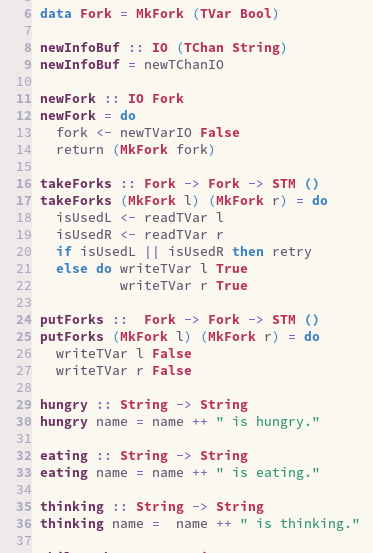
\includegraphics[width=8.5cm]{dinning1}}
      \centerline{ (a) Dinning Phhilosopher Part I}\medskip
    \end{minipage}
    \hfill
    \begin{minipage}[b]{0.48\linewidth}
      \centering
      \centerline{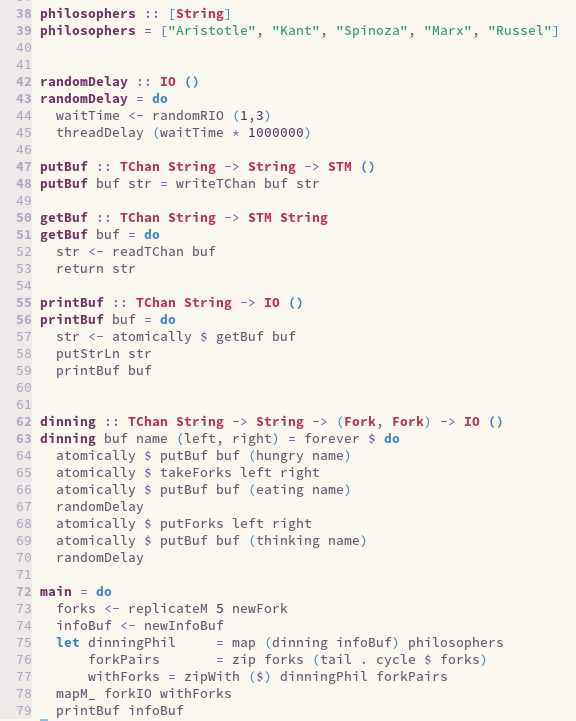
\includegraphics[width=8.5cm, height=12.5cm]{dinning2}}
      \centerline{ (b) Dinning Phhilosopher Part II }\medskip
    \end{minipage}
    \caption{Dinning Phhilosopher}
    \label{fig:dinning}
  \end{figure}

  Figure \ref{fig:dinning} contains two figures that show the full implementation of dinning philosopher using STM. Starting with figure
  \ref{fig:dinning} (a), the Fork type is defined with a constructor called
  MkFork which take a TVar with a Bool as an input. If the boolean inside the
  TVar is false then this fork is available to be used otherwise this fork is already taken. The newInfoBuf function will return a TChan with String wrapped in IO monad to be used later to store logs that indicate the running state of each thread. The newFork function will return a Fork wrapped in IO monad with the boolean value set to false.

  The next two function takeForks and putForks are related to require and release resources. The takeForks function takes two Fork as input. This function will first check if the two Forks are both available. The two Forks can only be used if they are both available at the same time. Otherwise, this function will keep retrying until both Forks can be required. The putForks function is simple just release the two Forks by setting the boolean to true.

  The next three functions hungry, eating, thinking are just dummy function that concatenates the name of the philosopher with corresponding information. This information will later be put into the infoBuf(TChan String). The names of philosophers are defined as a list of string as figure \ref{fig:dinning} (b)
  shows.

  The randomDelay function will call threadDelay to delay the running thread randomly from 1 to 3 seconds. The next three functions putBuf, getBuf printBuf are operations related to the infoBuf(TChan String) that is used to store the logs for running thread. The putBuf function will just store string to the infoBuf(TChan String), the getBuf function will return the string stored in TChan and wrap in STM monad. The printBuf will just print the string stored in TChan.

  The dinning function contains the implementation of dining philosophers. This function takes a TChan String(used to store logs), a string(indicates philosopher's names), and a pair of Fork as input. This function will first store a log in the TChan that indicates the philosopher is hungry. Then, this function will try to acquire the Fork using takeForks function. If the forks are acquired successfully, another log will be stored in the TChan that suggests the philosopher is eating. Followed by a random delay from 1 to 3 seconds, the forks will be released using putForks function and the corresponding log will be put into the TChan. Finally, the function ended with another random delay.

  The main function will first initialise 5 Forks using newFork function and an infoBuf using newInfoBuf functions. Then the philosophers' name will be bundled with the dinning function using the map function. Then, an infinite list of pair of forks will be generated such that each fork in the pair is distinct from the other. Followed by coupling pairs of forks with the dinning function, a list of runnable functions is made. Finally, the main function will run those function by mapping forkIO function to the runnable dining functions while the printBuf function is called to print the logs of those running thread.

   \begin{figure}[H]

    \begin{minipage}[b]{0.24\linewidth}
      \centering
      \centerline{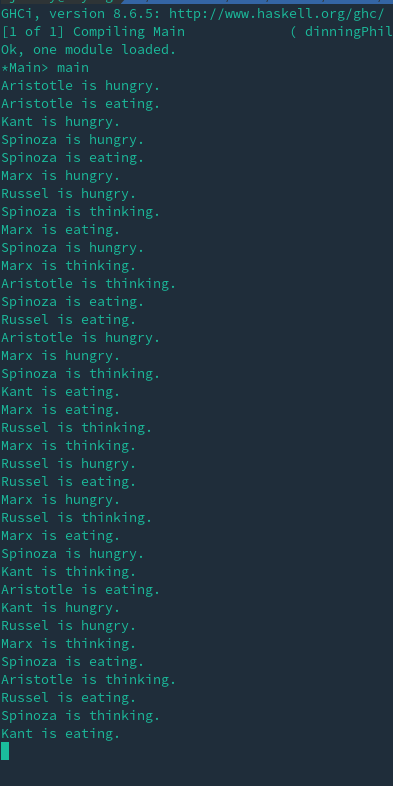
\includegraphics[width=4.0cm]{dinning10s}}
      \centerline{ (a) running at 10s}\medskip
    \end{minipage}
    \hfill
    \begin{minipage}[b]{0.24\linewidth}
      \centering
      \centerline{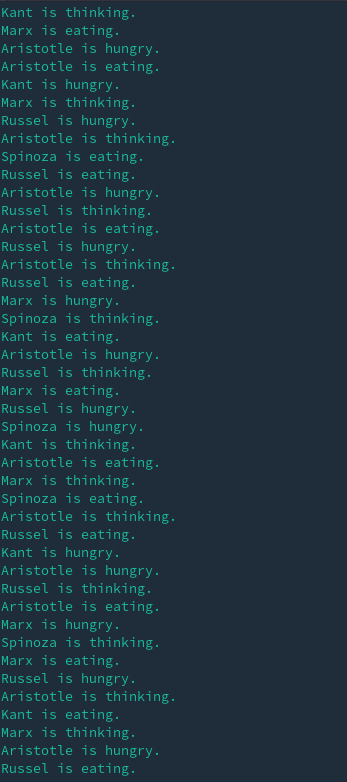
\includegraphics[width=4.0cm]{dinngin1m}}
      \centerline{ (b) running at 1m}\medskip
    \end{minipage}
    \hfill
    \begin{minipage}[b]{0.24\linewidth}
      \centering
      \centerline{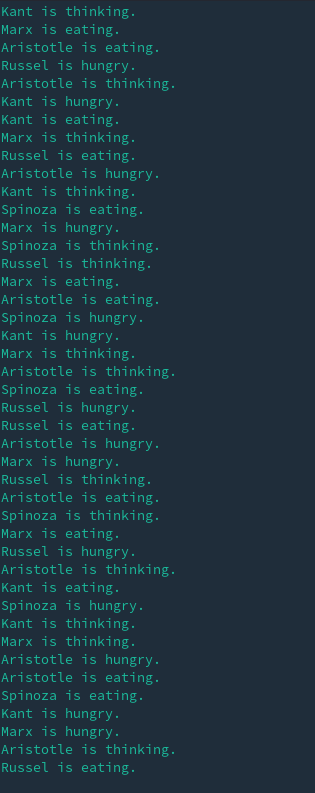
\includegraphics[width=4.0cm]{dinning2m}}
      \centerline{ (c) running at 2m}\medskip
    \end{minipage}
    \hfill
    \begin{minipage}[b]{0.24\linewidth}
      \centering
      \centerline{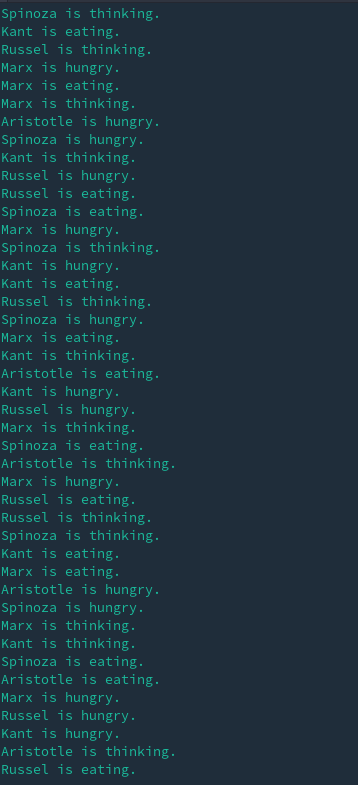
\includegraphics[width=4.0cm]{dinning4m}}
      \centerline{ (b) running at 4m}\medskip
    \end{minipage}

    \caption{Dinning Philosopher Running at Defferent Point of Time}
    \label{fig:drunning}
  \end{figure}

  Figure \ref{fig:drunning} contains four figures that shows this implementation
  running non-stop for four minutes. These sample output of the running program suggests that this implementation is working and without deadlocks. The main reason that this implementation is free of deadlocks is that it does not use locks at all and also this implementation uses STM which allows the threads running without the knowledge of the global environment. Giving two forks,
  each thread simple keep trying to acquire them at the same time until success. In this way, deadlocks can be avoided as resources will be acquired only until they are available. In contrast, if a thread acquired partially available and wait until another resource is available then deadlocks may easily occur.

  There are other solutions like resource hierarchy solution and arbitrator solution available for this problem. The resource hierarchy solution follows conventions that all forks are acquired in order and only one philosopher can pick up the fork in the highest order. This solution requires that all resources are known to all the philosophers. But this is often hard to achieve in real-world use cases which makes this solution impractical. As for the arbitrator solution, resource acquisition is controlled by an arbitrator instead of philosophers. While philosophers can put down forks at any time, the permission of picking up forks is controlled by the arbitrator and the arbitrator will grant the permission to only one philosopher at a time. One obvious issue for this solution is the permission control. All philosophers have to wait for permission from the arbitrator even if there are forks available. This issue would often cause efficiency problems.

  Comparing to those two solutions, STM solution is free of deadlocks and also the code is simple to write and expressive. But the STM solution is suffering from time penalty for committing atomic transactions. Also, one limitation of STM needs to be considered is that all the operations that can be performed by STM must be revertible. Despite its disadvantages and limits, STM is justified by its benefits.

  \section{Task II.2}
  Before the explanation of this implementation, the capabilities of this calculator will be introduced. The features supported by this calculator are:
  \begin{itemize}
  \item{Handle at least 10-digit integers}
  \item{Support addition, subtraction, multiplication, and division}
  \item{Allow the sign to be changed (+/-)}
  \item{Allow the calculator to be reset (C) as well as clearing the last
      entry (CE)}
  \item{Support calculations with decimal fractions (decimal point)}
  \item{Support standard precedence rules among the arithmetic operations
  along with parentheses for grouping}
  \item{Have a clearly structured implementation making use of functional
      reactive programming}
  \end{itemize}

  
  \begin{figure}[H]
    \centering
    \centerline{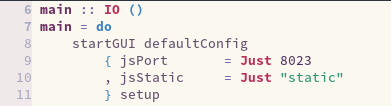
\includegraphics[scale=0.4]{calcmain}}
    \caption{Calculator Main Function}
    \label{fig:calcmain}
  \end{figure}

  Figure \ref{fig:calcmain} shows the main function of the calculator. This function is adopted from the examples provided by the threepenny library.

    \begin{figure}[H]

    \begin{minipage}[b]{0.48\linewidth}
      \centering
      \centerline{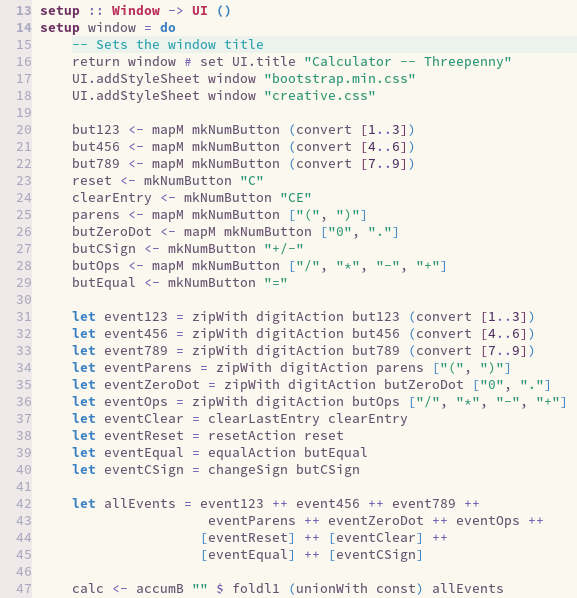
\includegraphics[width=8.5cm]{calcsetup1}}
      \centerline{ (a) Part I}\medskip
    \end{minipage}
    \hfill
    \begin{minipage}[b]{0.48\linewidth}
      \centering
      \centerline{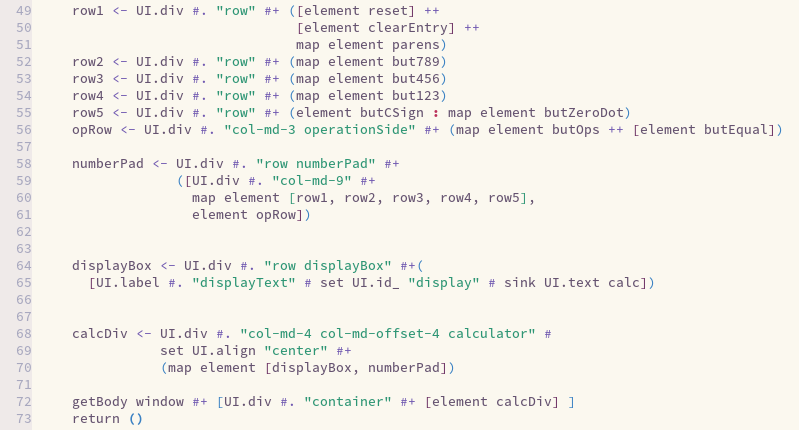
\includegraphics[width=8.5cm,height=5.5cm]{calcsetup2}}
      \centerline{ (b) Part II }\medskip
    \end{minipage}
    \caption{Calculator Setup Function}
    \label{fig:calcsetup}
  \end{figure}

  Figure \ref{fig:calcsetup} shows the implementation of setup function.
  The setup function is where logic and UI are defined. The first block of code in the setup function set the title of the window and imported two necessary CSS files for the layout. The first CSS file is the open source stylesheet called bootstrap that was developed by twitter. The second css \footnote[1]{https://github.com/xxczaki/calculator.js/blob/5d8ec0901e3503a6480d086df0d8e55c39908cdc/css/creative.css} file was obtained from GitHub to make the reasonable user interface. The next block contains the code of how the UI of all the buttons is created. The
  mkNumButton function is used for button creation. In general, buttons that same event function can be applied to can be created. However, in this case, buttons need to be created separately for layout arranging. For buttons that created together, mapM is used to apply mkNumButton function to all buttons with different id and text while a single button creation is using mkNumButton function directly.

  The on click events need to be coupled with buttons after all the buttons are created. This implementation using the parser for arithmetic expression recognition and evaluation. Therefore, all digit buttons,
  parentheses buttons, dot button and operation buttons(/, *, -, +) behave identically which is append text on the button to the existing input text. For all the button mentioned above, the digitAction function is used to handle the click event. The remaining buttons which are ce, reset, change sign and equal have different behaviours. Hence, each of them has a corresponding function defined to model their actions. Then, all buttons coupled with events are put in a list call allEvents. Finally, all the events are unified toghther with accumB function applied to. Until this point, all the core logics are embodied with buttons. The idea behind this embodiment is called functional reactive programming.

  The next part that is shown in figure \ref{fig:calcsetup} (b) is mostly the
  definition of UI components and their layout. The part begin with how buttons are grouped into different rows and then how numberPad of the calculator is formed by combining row. One of the most important UI component, displayBox, is defined here. All the result of button events and the result of evaluation of arithmetic expression will be displayed here. Therefore, all the logic parts are combined and applied here using sink function. Together with displayBox and numberPad, the definition of this calculator is completed. And finally, the displayBox and numberPad are displayed to the window.
  
  \begin{figure}[H]
    \centering
    \centerline{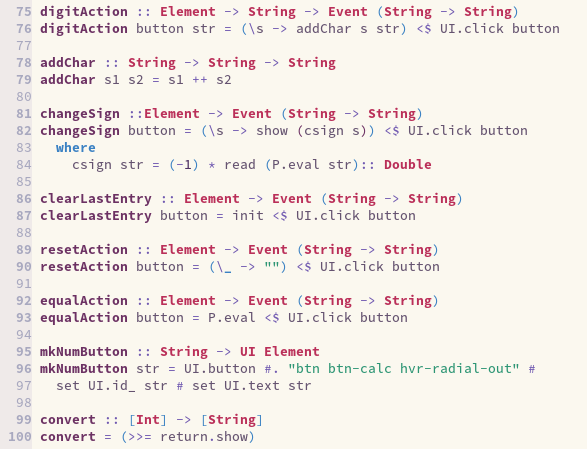
\includegraphics[scale=0.8]{calcfuncs}}
    \caption{Calculator Functions}
    \label{fig:calcfuncs}
  \end{figure}

  Figure \ref{fig:calcfuncs} shows functions related to button creation and button event mentioned earlier. The digitAction function takes a button and a string that is the button's text as input and return a function wrapped in Event as output. The function inside event takes the existing text as input and concatenate with the button's text and return the combined text. This is done through a dummy function called addChar.

  The changeSign function defined event related to change sign button. This function takes a button as input and will first calling the parser to evaluate the existing text(arithmetic expression) then change the sign of the evaluated result.

  Since all the inputs and the results are just strings. Therefore, the clear last entry can be implemented by simply calling the init function to remove the last bit. This is how the clearLastEntry function is defined.

  The reset event is even simpler than the clearLastEntry event. All the need to be done is discard everything by setting it to empty string.

  The final button event is the equalAction function. This function is simply passe the current input text to the parser for evaluation and returns the evaluated result.

  The mkNumButton function is used to create buttons. This function set the button id and display text according to the input string, and also some predefined class is set for layout purpose.
  
  Finally, a dummy function is defined to convert a list of integers to a list of corresponding strings.

  \begin{figure}[H]
    \begin{minipage}[b]{0.48\linewidth}
      \centering
      \centerline{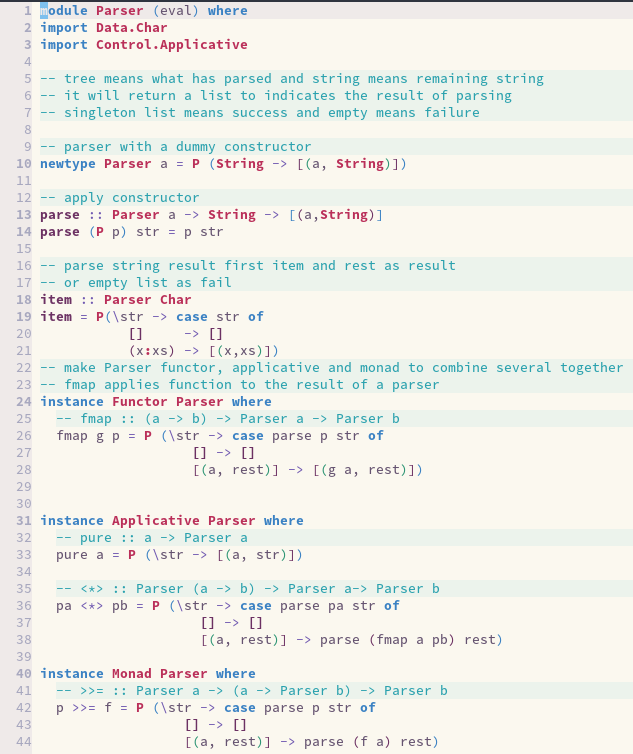
\includegraphics[width=8.5cm]{parserTypes}}
      \centerline{ (a) Parser Types}\medskip
    \end{minipage}
    \hfill
    \begin{minipage}[b]{0.48\linewidth}
      \centering
      \centerline{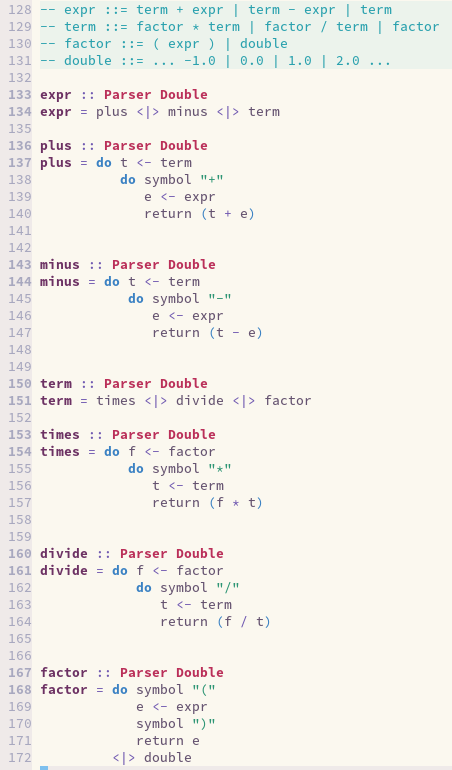
\includegraphics[width=8.5cm, height=10.5cm]{parserGrammar}}
      \centerline{ (b) Parser Grammer }\medskip
    \end{minipage}
    \caption{Parser}
    \label{fig:parser}
  \end{figure}

  The calculator is implemented by using a parser to evaluate the arithmetic expressions and return the results. Figure \ref{fig:parser} shows part of the parser type definition and how the arithmetic expressions are defined in context-free grammar and then converted to Haskell code.

  \begin{figure}[H]
    \centering
    \centerline{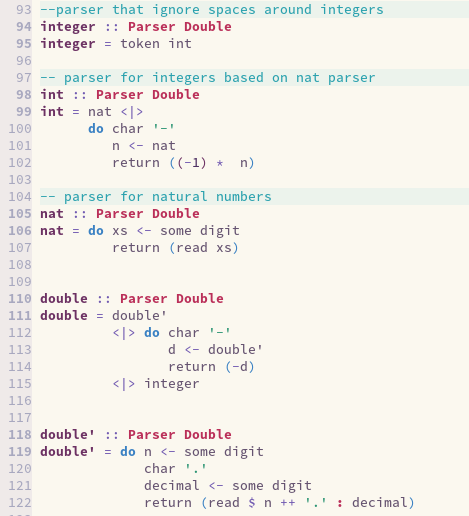
\includegraphics[scale=0.8]{parserDouble}}
    \caption{Parse Doubles}
    \label{fig:parseDouble}
  \end{figure}

  This parser implementation is inspired by Graham Hutton in his book called Programming in Haskell. Most of this parser is identical to Hutton's implementation which has a thorough introduction in his book. But how to parse floating number is not mentioned. Figure \ref{fig:parseDouble} contains a novel implementation
  of how to parse floating numbers from string. And this part is essential to ensure the functionality of the calculator.

  Finally, the following figures are screenshots that show the calculator in action.

  \begin{figure}[H]
    \begin{minipage}[b]{0.48\linewidth}
      \centering
      \centerline{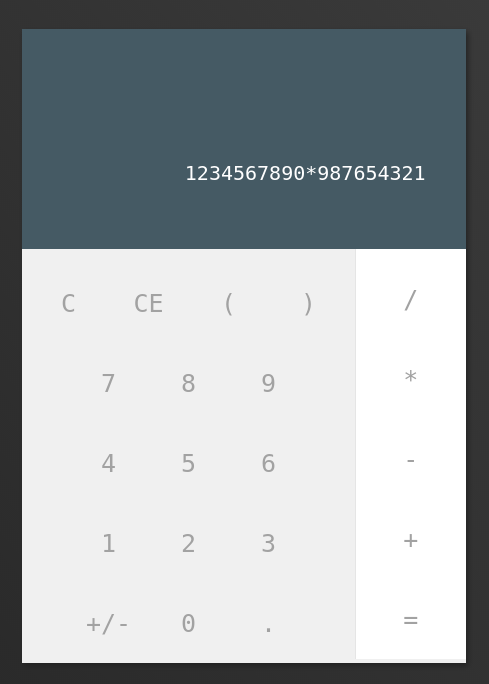
\includegraphics[width=8.5cm]{10*}}
      \centerline{ (a) Integer Multiplication }\medskip
    \end{minipage}
    \hfill
    \begin{minipage}[b]{0.48\linewidth}
      \centering
      \centerline{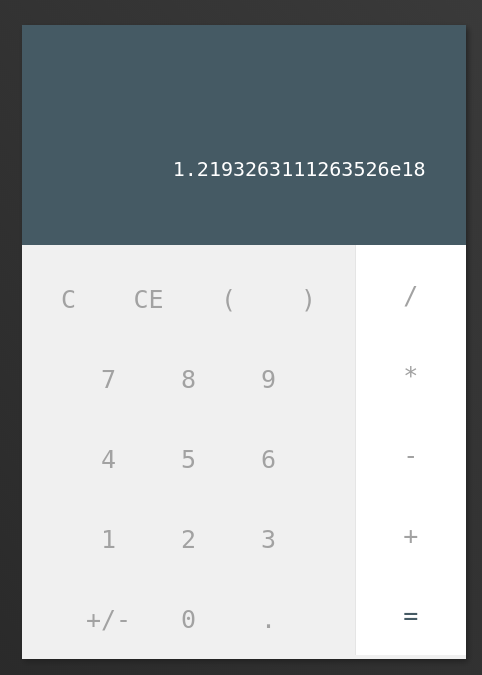
\includegraphics[width=8.5cm]{10*res}}
      \centerline{ (b) Result }\medskip
    \end{minipage}
    \caption{Integer Multiplication}
  \end{figure}

  \begin{figure}[H]
    \begin{minipage}[b]{0.48\linewidth}
      \centering
      \centerline{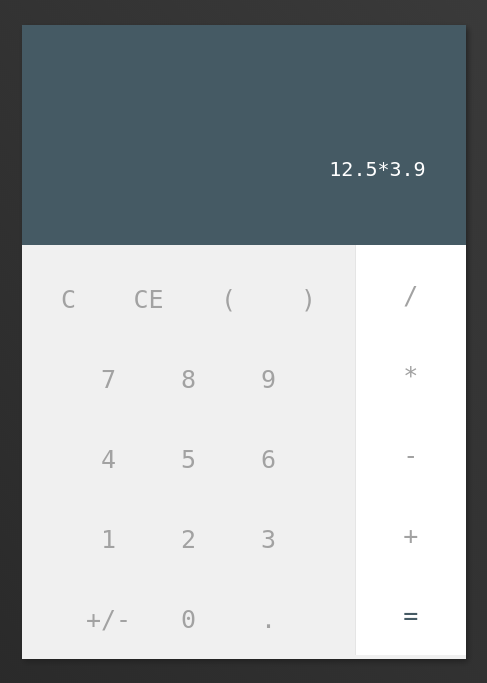
\includegraphics[width=8.5cm]{dec*}}
      \centerline{ (a) Decimal Fractions Multiplication }\medskip
    \end{minipage}
    \hfill
    \begin{minipage}[b]{0.48\linewidth}
      \centering
      \centerline{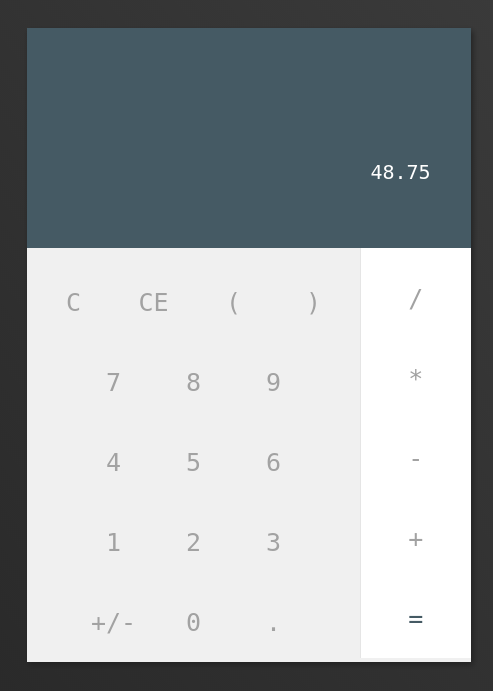
\includegraphics[width=8.5cm]{dec*res}}
      \centerline{ (b) Result }\medskip
    \end{minipage}
    \caption{Decimal Fractions Multiplication}
  \end{figure}

  
  \begin{figure}[H]
    \begin{minipage}[b]{0.48\linewidth}
      \centering
      \centerline{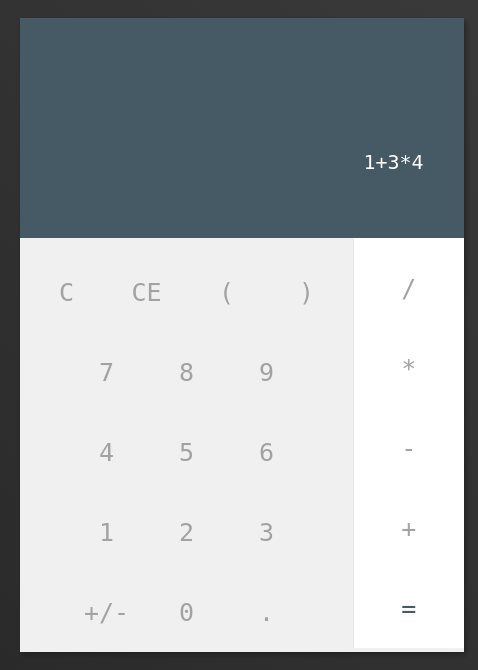
\includegraphics[width=8.5cm]{134}}
      \centerline{ (a) Precedence Rules }\medskip
    \end{minipage}
    \hfill
    \begin{minipage}[b]{0.48\linewidth}
      \centering
      \centerline{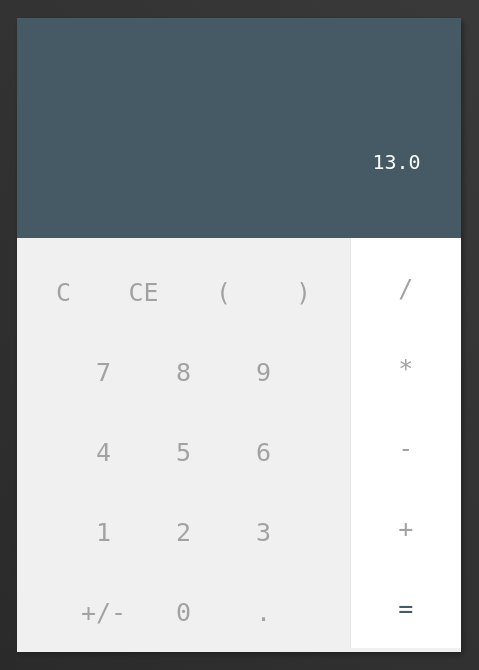
\includegraphics[width=8.5cm]{134res}}
      \centerline{ (b) Result }\medskip
    \end{minipage}
    \caption{Precedence Rules}
  \end{figure}

  
  \begin{figure}[H]
    \begin{minipage}[b]{0.48\linewidth}
      \centering
      \centerline{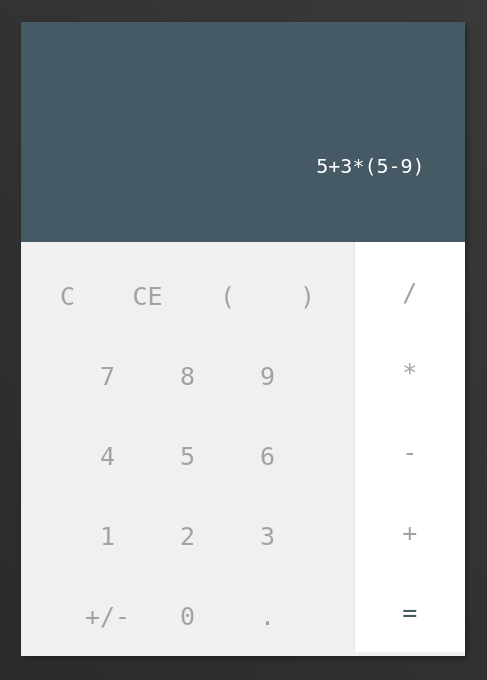
\includegraphics[width=8.5cm]{5-3*(5-9)}}
      \centerline{ (a) Paretheses Grouping }\medskip
    \end{minipage}
    \hfill
    \begin{minipage}[b]{0.48\linewidth}
      \centering
      \centerline{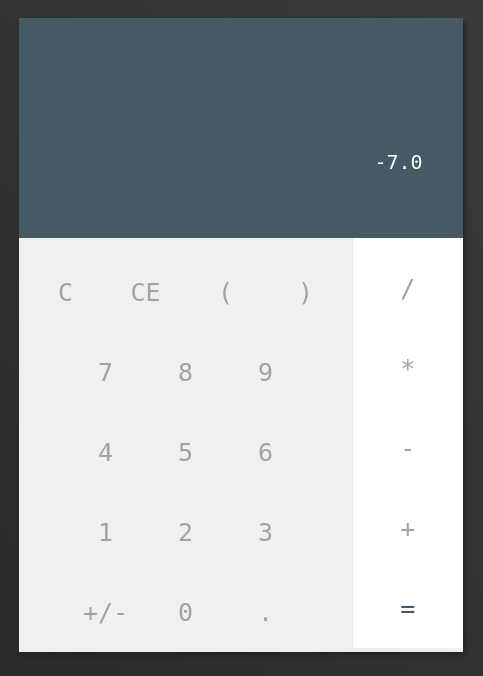
\includegraphics[width=8.5cm]{5-3*(5-9)res}}
      \centerline{ (b) Result }\medskip
    \end{minipage}
    \caption{Paretheses Grouping}
  \end{figure}

  
\end{document}
